\documentclass[12pt,letterpaper]{article}
\usepackage[utf8]{inputenc}
\usepackage[spanish,es-tabla]{babel}
\usepackage[margin=2.54cm]{geometry}
\usepackage{mathptmx} 
\usepackage{tabularx}
\usepackage{xltabular}

\renewcommand{\labelitemi}{\textbullet}

% Interlineado doble y sangría de primera línea (0.5 pulgadas = 1.27 cm)
\usepackage{setspace}
%\doublespacing
\setlength{\parindent}{1.27cm}
\setlength{\parskip}{0pt}
\usepackage{ragged2e}
\usepackage{sectsty}
\allsectionsfont{\raggedright}

\usepackage{fancyhdr}
\pagestyle{fancy}
\fancyhf{}
\fancyfoot[C]{\thepage}
\renewcommand{\headrulewidth}{0pt}
\usepackage{enumitem}
\usepackage{array}
\usepackage{graphicx}
\usepackage{float}
\usepackage{amsmath}

\setcounter{secnumdepth}{2}
\setcounter{tocdepth}{2}
\graphicspath{{Imagenes/}} 

\begin{document}
% --- caratula ---
\begin{titlepage}
    \centering
    
    {\bfseries\large UNIVERSIDAD MAYOR DE SAN ANDRÉS\par}
    \vspace{0.4cm} 
    
    {\bfseries\large FACULTAD DE CIENCIAS PURAS Y NATURALES\par}
    \vspace{0.2cm}
    
    
    % Logo UMSA 
    
\includegraphics[width=3cm]{Umsa-logo.png}\par
    \vspace{1cm}
    
    % Título del proyecto
    {\bfseries\Large Sistema de compra de materiales de escritorio\par}
    {\bfseries\large Caso: Importadora “Suministros G\&T”\\}
    
    \vfill 

    \begin{flushleft}
    \hspace{2.2cm} % Ajustado ligeramente para que entren los nombres largos sin desbordarse
    \begin{tabular}{ll}
        \textbf{Asignatura:}  & Ingeniería de Software II \\[0.4em]
        \textbf{Sigla:}       & INF-261 \\[0.4em]
        \textbf{Integrantes:} & Univ. Quispe Gutierrez Carla Ines \\
                              & Univ. Mamani Chavez Rafael Alejandro \\
                              & Univ. Quispe Huanca Iver \\
                              & Univ. Quispe Choque Ivone \\
                              & Univ. Herrera Sirpa Jesús Abed \\
                              & Univ. Condori Quispe Rocío \\
                              & Univ. Laura Mamani Alvaro Luis \\[1.2em]
        \textbf{Docente:}     & M. Sc. German Huanca Ticona \\[0.6em]
    %   \textbf{Fecha:}       & \today
    \end{tabular}
    \end{flushleft}
    
    \vfill
    
    {\bfseries LA PAZ -- BOLIVIA\par}

\end{titlepage}
\newpage

\thispagestyle{empty}
\tableofcontents
\newpage

% --- Reiniciar numeración en la Introducción ---
\pagenumbering{arabic}
\setcounter{page}{1}

% --- Secciones ---
% --- Introducción ---
\section{Introducción}

En el entorno comercial actual, la digitalización de los procesos de venta y atención al cliente constituye un factor determinante para la competitividad de las empresas distribuidoras. Las organizaciones dedicadas a la comercialización de materiales de escritorio y papelería enfrentan el desafío constante de gestionar catálogos amplios con alta rotación de inventario, donde la dependencia de registros manuales o la atención exclusivamente presencial puede derivar en demoras operativas, desactualización de precios y errores en el control de existencias.

El presente documento desarrolla la especificación de ingeniería de software para el \textbf{Sistema Web de Compra de Materiales de Escritorio}, orientado al modelo de negocio B2C (\textit{Business to Consumer}), para la empresa importadora y comercializadora \textbf{``Suministros G\&T''}. El propósito de esta solución es modernizar el canal de ventas mediante una plataforma virtual intuitiva que permita a los clientes particulares y oficinistas explorar el catálogo digital por categorías, consultar disponibilidad en tiempo real, gestionar su carrito de compras y confirmar pedidos, al tiempo que dota al administrador de herramientas centralizadas para el control de productos, inventario y estados de entrega.

\subsection{Planteamiento del Problema}

Actualmente, la gestión comercial de ``Suministros G\&T'' presenta limitaciones propias de los procesos tradicionales: la consulta de disponibilidad de artículos y precios requiere intervención directa del personal de tienda, lo que ralentiza la toma de pedidos y dificulta la atención simultánea de múltiples clientes. Asimismo, la falta de una sincronización automatizada entre las solicitudes de compra y el inventario físico incrementa el riesgo de comprometer artículos sin existencias (\textit{stock}) o de mantener información desactualizada en el catálogo.

Ante esta situación, surge la necesidad de diseñar una plataforma web cliente-servidor que centralice la información comercial, automatice el cálculo de importes y la validación de existencias antes de confirmar cada pedido, y proporcione trazabilidad tanto al comprador como al equipo administrativo.

\subsection{Objetivos del Proyecto}

\subsubsection{Objetivo General}
Elaborar el análisis, planificación y modelado técnico detallado del Sistema Web de Compra de Materiales de Escritorio bajo el modelo B2C para la empresa ``Suministros G\&T'', aplicando las prácticas del Proceso Unificado Ágil (AUP) para garantizar una especificación consistente, trazable y orientada a la calidad del software.

\subsubsection{Objetivos Específicos}
\begin{itemize}
    \item Identificar los actores principales y de contexto que interactúan con la plataforma, así como especificar y codificar los 18 requerimientos funcionales (\texttt{RF01}--\texttt{RF18}) y 11 requerimientos no funcionales (\texttt{RNF01}--\texttt{RNF11}) del sistema.
    \item Delimitar el alcance técnico del proyecto hasta la fase de diseño detallado, estableciendo la estructura de roles del equipo, la estimación de esfuerzo, el cronograma iterativo y la matriz de gestión de riesgos (RMMM).
    \item Modelar el comportamiento dinámico, la estructura lógica, el esquema relacional de base de datos en MySQL y los prototipos visuales (UX/UI) que cubran al $100\%$ los requerimientos establecidos.
    \item Asegurar la calidad y consistencia de todos los artefactos mediante mecanismos de control de configuración en GitHub, auditorías UML y una matriz de trazabilidad requerimiento-modelo.
\end{itemize}

\subsection{Estructura del Documento}

Para abordar de manera ordenada las etapas iniciales del ciclo de vida del software, el presente informe se organiza en cuatro secciones principales:
\begin{itemize}
    \item \textbf{Introducción:} Contextualiza la problemática comercial de ``Suministros G\&T'', plantea los objetivos general y específicos, y describe la organización del documento.
    \item \textbf{Marco Teórico y Metodología (AUP):} Expone los fundamentos del Proceso Unificado Ágil (\textit{Serial in the Large} e \textit{Iterative in the Small}), sus ventajas para el sector papelero, las herramientas de modelado y arquitectura de referencia, y las políticas de gestión de configuración.
    \item \textbf{Fase I: Comunicación:} Detalla la identificación de actores, el catálogo completo de requerimientos funcionales y no funcionales, el glosario técnico del dominio y el modelado general y expandido de casos de uso.
    \item \textbf{Fase II: Planeación:} Define los límites y exclusiones del alcance, la asignación de roles del equipo de siete integrantes, la estimación de esfuerzo en horas-persona, el cronograma de tres iteraciones, la estrategia de riesgos RMMM, los mecanismos de auditoría y los criterios de aceptación.
\end{itemize}
% --- Marco teórico y metodología ---
\section{Marco Teórico y Metodología (AUP)}

El presente proyecto se fundamenta en el Proceso Unificado Ágil (\textit{Agile Unified Process}, AUP), una metodología híbrida propuesta por Scott Ambler que simplifica el Proceso Unificado de Rational (RUP) mediante la incorporación de prácticas ágiles como el modelado ágil, la validación continua y la gestión controlada de cambios. Su objetivo es proporcionar un marco estructurado pero ligero que permita especificar y diseñar software de alta calidad sin burocracia excesiva.

\subsection{Agile Unified Process (AUP)}

AUP organiza el ciclo de vida del desarrollo de software en cuatro fases secuenciales -Inicio, Elaboración, Construcción y Transición-, mientras ejecuta de manera iterativa siete disciplinas clave (Modelo, Implementación, Prueba, Despliegue, Gestión de Configuración, Gestión de Proyectos y Entorno) dentro de cada iteración. Considerando el alcance académico del proyecto, el equipo aplica las disciplinas de Modelo, Gestión de Configuración y Gestión de Proyectos a lo largo de las fases de Inicio (Comunicación y Planeación) y Elaboración (Modelado detallado), dejando las fases de Construcción y Transición proyectadas para una etapa posterior de implementación.

\subsubsection{Filosofía \textit{Serial in the Large} e \textit{Iterative in the Small}}

La arquitectura metodológica de AUP se sustenta en un principio dual que equilibra la planificación macro con la agilidad operativa:

\begin{itemize}
    \item \textbf{\textit{Serial in the Large} (En serie a gran escala):} A nivel global del proyecto, las fases principales se ejecutan de manera secuencial. Esto garantiza que se establezcan hitos claros de control, líneas base aprobadas (\texttt{LB-I1}, \texttt{LB-I2}, \texttt{LB-I3}) y una visión arquitectónica sólida antes de comprometer recursos en etapas posteriores.
    \item \textbf{\textit{Iterative in the Small} (Iterativo a pequeña escala):} Dentro de cada fase, el trabajo se divide en iteraciones cortas e incrementales. En cada iteración el equipo refina los modelos, valida los requerimientos, actualiza la arquitectura y verifica la consistencia de los artefactos, permitiendo adaptarse rápidamente a hallazgos o ajustes del negocio sin perder el rumbo general.
\end{itemize}

\subsubsection{Ventajas para el sector industrial (Papelero)}

La aplicación de AUP en el contexto comercial del sector papelero y de suministros de oficina -específicamente para la empresa ``Suministros G\&T''- ofrece beneficios estratégicos directos:

\begin{itemize}
    \item \textbf{Control preciso de catálogos e inventarios:} El sector papelero maneja una alta variedad de artículos (cuadernos, papelería bond, escritura, archivo) con rotación constante. El modelado iterativo permite validar tempranamente las reglas de negocio críticas, como el descuento automático de \textit{stock} al confirmar pedidos y la prevención de ventas sin existencias.
    \item \textbf{Trazabilidad y estandarización:} La disciplina de Gestión de Configuración asegura que los cambios en requerimientos, categorías o flujos de pedido queden documentados y vinculados desde la especificación hasta el diseño de base de datos, evitando inconsistencias operativas.
    \item \textbf{Reducción de riesgos en la digitalización comercial:} Al transicionar de procesos manuales hacia una plataforma web B2C (\textit{Business to Consumer}), AUP permite validar los flujos de compra y prototipos visuales desde las primeras semanas, garantizando una interfaz intuitiva tanto para compradores particulares como para administradores de tienda.
\end{itemize}

\subsection{Tecnologías y Herramientas Propuestas}

Para el diseño del Sistema Web de Compra de Materiales de Escritorio de la empresa ``Suministros G\&T'' se define una arquitectura cliente-servidor orientada al comercio electrónico B2C, que permite centralizar la gestión del catálogo, carrito de compras, control de inventario y seguimiento de pedidos.

En concordancia con el alcance establecido en la Sección \ref{subsec:alcance_delimitacion}, la Tabla \ref{tab:tecnologias_herramientas} distingue tanto las herramientas utilizadas directamente en las fases de análisis, modelado y prototipado como el \textit{stack} tecnológico de referencia sobre el cual se especifican la arquitectura y el diccionario de datos para su futura implementación.

{\small
\begin{xltabular}{\textwidth}{|>{\raggedright\arraybackslash}p{2.8cm}|>{\raggedright\arraybackslash}p{3.4cm}|X|}
    \caption{Tecnologías y herramientas de modelado y arquitectura de referencia}
    \label{tab:tecnologias_herramientas} \\
    \hline
    \textbf{Elemento} & \textbf{Herramienta propuesta} & \textbf{Justificación} \\
    \hline
    \endfirsthead

    \multicolumn{3}{l}{\textit{Continuación de la Tabla \ref{tab:tecnologias_herramientas}}} \\
    \hline
    \textbf{Elemento} & \textbf{Herramienta propuesta} & \textbf{Justificación} \\
    \hline
    \endhead

    \multicolumn{3}{r}{\textit{Continúa en la siguiente página...}} \\
    \endfoot

    \endlastfoot

    Modelado UML y de datos & Draw.io (diagrams.net) & Herramienta estandarizada del equipo para elaborar todos los diagramas UML (casos de uso, clases, secuencia, actividades, estados, componentes y despliegue) y el modelo E-R. \\*
    \hline
    Diseño de prototipos & Figma & Permite diseñar los \textit{wireframes} y \textit{mockups} navegables de las interfaces de Cliente y Administrador para validar la experiencia de usuario (UX/UI). \\*
    \hline
    Control de versiones & Git y GitHub & Permiten centralizar los archivos editables (\texttt{.drawio}, \texttt{.tex}), gestionar ramas por artefacto y auditar el historial de cambios del equipo. \\*
    \hline
    Documentación técnica & Overleaf (LaTeX) & Permite redactar, estructurar y compilar de forma colaborativa el informe técnico maestro bajo estándares formales. \\*
    \hline
    Base de datos (especificación) & MySQL & Motor relacional de referencia utilizado para definir los tipos de datos, restricciones de integridad y esquema normalizado en el diccionario de datos. \\*
    \hline
    Interfaz de usuario (referencia) & HTML5, CSS3, JavaScript y Bootstrap & Tecnologías proyectadas para construir una interfaz web responsiva e intuitiva en la etapa posterior de desarrollo. \\*
    \hline
    Backend / Lógica (referencia) & Node.js (Express) & Entorno proyectado para centralizar las reglas de negocio del modelo B2C, la autenticación por roles y las validaciones de inventario. \\
    \hline
\end{xltabular}
}

Estas herramientas garantizan una especificación técnica organizada, trazable y consistente durante las fases de Comunicación, Planeación y Modelado, sentando bases sólidas para una futura fase de construcción sin ambigüedades.

\subsection{Gestión de la Configuración y Documentación}

La gestión de la configuración es una actividad fundamental para mantener el control de los cambios realizados durante el análisis y modelado del Sistema Web de Compra de Materiales de Escritorio para ``Suministros G\&T''. Esta disciplina permite organizar y auditar las diferentes versiones de los diagramas, esquemas de base de datos, prototipos y documentación técnica del proyecto.

Para llevar un adecuado control de la configuración se establecen las siguientes actividades:

\begin{itemize}
    \item \textbf{Crear un repositorio del proyecto:} Utilizar GitHub para centralizar todos los archivos del equipo y mantener un respaldo seguro. Se organizarán carpetas estructuradas como \texttt{/docs}, \texttt{/diagramas}, \texttt{/bd} y \texttt{/prototipos}.
    \item \textbf{Definir ramas de trabajo:} Utilizar la rama \texttt{main} para las líneas base aprobadas, \texttt{develop} para integrar los avances validados y ramas \texttt{feature} por artefacto o módulo (por ejemplo, \texttt{feature/diagrama-clases} o \texttt{feature/modelo-er}).
    \item \textbf{Registrar los cambios realizados:} Utilizar Git para guardar las modificaciones mediante mensajes descriptivos estandarizados, por ejemplo: ``\texttt{docs: actualizar requerimientos funcionales}'', ``\texttt{feat: agregar diagrama de secuencia carrito}'' o ``\texttt{fix: corregir cardinalidad en modelo ER}''.
    \item \textbf{Controlar las versiones del esquema de base de datos:} Mantener scripts SQL de especificación numerados para registrar la evolución del diseño relacional, por ejemplo: \texttt{V01\_esquema\_tablas.sql} y \texttt{V02\_restricciones\_fk.sql}.
    \item \textbf{Mantener un registro de modificaciones:} Utilizar un archivo \texttt{CHANGELOG.md} donde se registren las fechas, responsables y descripciones de los cambios aprobados en cada iteración.
    \item \textbf{Controlar las versiones de documentos:} Etiquetar las entregas del documento maestro mediante las líneas base planificadas (\texttt{LB-I1}, \texttt{LB-I2} y \texttt{LB-I3}), evitando la duplicación o pérdida de avances.
    \item \textbf{Aprobar cambios en los requerimientos:} Cualquier solicitud de modificación tras cerrar \texttt{LB-I1} deberá registrarse indicando su descripción, motivo, impacto en los modelos, responsable y aprobación del Coordinador y QA.
    \item \textbf{Elaborar documentación técnica:} Mantener actualizados los casos de uso expandidos, el glosario técnico, el diccionario de datos, los diagramas UML y la matriz de trazabilidad.
\end{itemize}

Para mantener una adecuada organización, en la Tabla \ref{tab:control_artefactos} se establece el esquema de control de los principales artefactos del proyecto.

{\small
\begin{xltabular}{\textwidth}{|>{\raggedright\arraybackslash}p{3.2cm}|>{\raggedright\arraybackslash}p{3.4cm}|X|}
    \caption{Control de artefactos principales del proyecto}
    \label{tab:control_artefactos} \\
    \hline
    \textbf{Artefacto} & \textbf{Responsable sugerido} & \textbf{Control requerido} \\
    \hline
    \endfirsthead

    \multicolumn{3}{l}{\textit{Continuación de la Tabla \ref{tab:control_artefactos}}} \\
    \hline
    \textbf{Artefacto} & \textbf{Responsable sugerido} & \textbf{Control requerido} \\
    \hline
    \endhead

    \multicolumn{3}{r}{\textit{Continúa en la siguiente página...}} \\
    \endfoot

    \endlastfoot

    Documento maestro & Líder de proyecto / Coordinador & Control de versiones (\texttt{LB-I1} a \texttt{LB-I3}), fechas de actualización y consolidación del texto. \\*
    \hline
    Diagramas UML & Especialistas en modelado dinámico y estructural & Mantener archivos editables (\texttt{.drawio}), exportaciones PNG/PDF y coherencia con la plantilla visual. \\*
    \hline
    Modelo de datos & Especialistas en modelado estructural y BD & Control del modelo E-R, esquema relacional normalizado, diccionario de datos y scripts SQL de referencia. \\*
    \hline
    Prototipos de interfaz & Especialista en arquitectura y UX/UI & Mantener actualizados los \textit{wireframes} y \textit{mockups} navegables en Figma según los RF/RNF. \\*
    \hline
    Auditoría y trazabilidad & Responsable de calidad (QA) & Gestionar la matriz de trazabilidad al $100\%$, actas de revisión y control de ramas en GitHub. \\
    \hline
\end{xltabular}
}

La aplicación de estas actividades permitirá mantener la organización del proyecto, facilitar el trabajo colaborativo entre los siete integrantes y garantizar que todos los artefactos estén debidamente versionados y controlados durante las fases abordadas bajo la metodología AUP.
% --- Comunicación ---
\section{Fase I: Comunicación}

La fase de comunicación, denominada también fase de Inicio o Concepción en el Proceso Unificado Ágil (AUP), representa el punto de partida fundamental de todo el ciclo de vida del software. Según lo establece Roger S. Pressman en su obra \textit{Ingeniería del Software: Un enfoque práctico}, esta actividad estructural tiene como objetivo principal fomentar la colaboración entre el equipo de desarrollo y los interesados (\textit{stakeholders}) para comprender las necesidades reales de la tienda comercializadora y de los clientes que utilizarán la plataforma.

Para el proyecto ``Sistema Web de Compra de Materiales de Escritorio para la empresa Suministros G\&T'', esta fase se orienta bajo el modelo de negocio B2C (\textit{Business to Consumer}), permitiendo que la empresa ofrezca sus productos directamente a clientes particulares a través de una tienda virtual. Mediante un proceso riguroso de indagación y análisis, se identifican los actores involucrados, se establecen los requerimientos funcionales y no funcionales, se definen los términos clave del dominio y se modela el comportamiento general del sistema mediante casos de uso.

\subsection{Identificación de Actores}

Un actor representa cualquier entidad externa (persona, departamento o sistema) que interactúa directamente con la plataforma o que posee un interés directo en su funcionamiento y resultados. Para el sistema web de ``Suministros G\&T'', se han identificado y clasificado los siguientes actores principales y de contexto:

\begin{itemize}
    \item \textbf{Cliente (Comprador Particular u Oficinista):} Es el actor principal del modelo B2C. Representa a la persona natural que accede a la tienda virtual para registrarse, iniciar sesión, consultar el catálogo digital, buscar materiales de escritorio (cuadernos, bolígrafos, papel, archivadores, etc.), revisar características y precios actualizados, administrar su carrito de compras y confirmar pedidos de manera segura.
    \item \textbf{Administrador del Sistema (Gerente de Tienda o Encargado de Inventario):} Es el responsable de gestionar la operatividad comercial de la plataforma. Cuenta con privilegios elevados para registrar, modificar o desactivar productos, organizar categorías, actualizar precios y existencias (\textit{stock}) en tiempo real, administrar cuentas de usuario y supervisar el flujo y estado de los pedidos realizados por los clientes.
    \item \textbf{Proveedor (Actor Externo de Contexto):} Aunque no interactúa directamente con la interfaz del software, constituye una entidad fundamental en el ecosistema del negocio al abastecer de materiales a ``Suministros G\&T''. El sistema refleja este flujo mediante el control de inventario para garantizar la disponibilidad física de los artículos ofertados.
    \item \textbf{Equipo de Desarrollo (Analistas, Diseñadores y Programadores):} Los integrantes del equipo de Ingeniería de Software actúan como los responsables de analizar, diseñar, construir y documentar la solución técnica, asegurando el cumplimiento de los estándares de calidad y los plazos establecidos.
    \item \textbf{Docente de la Asignatura (Cliente Académico / Evaluador):} Actúa como \textit{stakeholder} auditor del proceso, verificando que la aplicación de las metodologías de ingeniería de software (AUP y Pressman) se ejecute de forma rigurosa y debidamente documentada.
\end{itemize}

\subsection{Requerimientos Funcionales y No Funcionales}

A través del análisis del negocio se han extraído y codificado los requerimientos del sistema para garantizar su trazabilidad durante todo el ciclo de desarrollo.

\subsubsection{Requerimientos Funcionales (RF)}

Los requerimientos funcionales describen las operaciones, validaciones y servicios específicos que la plataforma debe ofrecer a sus usuarios:

\begin{itemize}
    \item \textbf{RF01 (Registro de clientes):} El sistema permitirá a los nuevos usuarios crear una cuenta mediante un formulario, registrando y validando sus datos básicos (nombre, correo electrónico, dirección, teléfono y contraseña).
    \item \textbf{RF02 (Inicio y cierre de sesión):} El sistema permitirá a los usuarios registrados (clientes y administradores) autenticarse mediante credenciales válidas, redirigiéndolos a su entorno correspondiente, así como cerrar su sesión de forma segura.
    \item \textbf{RF03 (Gestión de perfiles):} El cliente autenticado podrá consultar su información personal y actualizar datos como su dirección, teléfono o contraseña.
    \item \textbf{RF04 (Catálogo digital de productos):} El sistema mostrará un catálogo digital organizado con los materiales de escritorio disponibles en la tienda (cuadernos, bolígrafos, lápices, hojas bond, carpetas, archivadores, marcadores, entre otros).
    \item \textbf{RF05 (Clasificación por categorías):} El sistema permitirá filtrar y navegar los productos agrupados en categorías lógicas para facilitar su localización.
    \item \textbf{RF06 (Búsqueda de productos):} El cliente podrá buscar artículos específicos ingresando palabras clave, nombre del producto o categoría en un buscador interno.
    \item \textbf{RF07 (Detalle del producto):} Al seleccionar un artículo, el cliente podrá visualizar una ficha informativa con su nombre, descripción detallada, características, precio unitario, imagen referencial y disponibilidad (\textit{stock}).
    \item \textbf{RF08 (Carrito de compras):} El sistema permitirá al cliente seleccionar la cantidad deseada de un producto y agregarlo a un carrito de compras virtual.
    \item \textbf{RF09 (Modificación del carrito):} El cliente podrá modificar las cantidades de los artículos añadidos al carrito o eliminarlos antes de confirmar su pedido.
    \item \textbf{RF10 (Cálculo automático de importes):} El sistema calculará en tiempo real los subtotales por cada producto y el monto total general de la compra conforme se modifica el carrito.
    \item \textbf{RF11 (Validación de disponibilidad):} El sistema validará que las cantidades solicitadas sean válidas y que exista \textit{stock} suficiente en el inventario antes de permitir la confirmación de un pedido.
    \item \textbf{RF12 (Confirmación y registro de pedidos):} El cliente podrá revisar el resumen de su compra y confirmar el pedido, generando un registro único con el detalle de productos, cantidades, precios, fecha y datos del comprador, descontando automáticamente las existencias.
    \item \textbf{RF13 (Historial y seguimiento de pedidos):} El cliente podrá consultar su historial de compras realizadas y visualizar el estado actual de sus pedidos vigentes (ej. ``Recibido'', ``En preparación'', ``En camino'', ``Entregado'').
    \item \textbf{RF14 (Administración de productos):} El administrador contará con un módulo para registrar nuevos productos, consultar y modificar los existentes (precios, descripciones, imágenes) y desactivar aquellos que ya no se comercialicen.
    \item \textbf{RF15 (Administración de categorías):} El administrador podrá crear, modificar, organizar y desactivar las categorías de productos del catálogo.
    \item \textbf{RF16 (Gestión de precios e inventario):} El administrador podrá actualizar los precios y reabastecer las existencias (\textit{stock}) de los materiales para mantener la sincronía con el almacén físico.
    \item \textbf{RF17 (Gestión de pedidos):} El administrador podrá consultar todos los pedidos realizados por los clientes, revisar su detalle y actualizar su estado de atención y entrega.
    \item \textbf{RF18 (Gestión de usuarios):} El administrador podrá consultar el listado de clientes registrados y administrar el estado de sus cuentas dentro de la plataforma.
\end{itemize}

\subsubsection{Requerimientos No Funcionales (RNF)}

Los requerimientos no funcionales establecen los atributos de calidad, restricciones técnicas y estándares de operación que debe cumplir la plataforma:

\begin{itemize}
    \item \textbf{RNF01 (Usabilidad):} La interfaz debe ser clara, ordenada e intuitiva, aplicando principios de diseño UX/UI para facilitar la navegación y minimizar la curva de aprendizaje tanto para clientes como para administradores.
    \item \textbf{RNF02 (Rendimiento):} Las consultas al catálogo, búsquedas y operaciones del carrito deberán responder en tiempos óptimos (menores a 3 segundos en condiciones normales) para brindar una experiencia fluida.
    \item \textbf{RNF03 (Seguridad y control de acceso):} El sistema protegerá el acceso mediante autenticación robusta y restringirá las funciones administrativas exclusivamente a usuarios con el rol autorizado.
    \item \textbf{RNF04 (Privacidad y protección de datos):} Las contraseñas y datos personales de los clientes se almacenarán de forma cifrada y se utilizarán únicamente para las operaciones propias de la tienda virtual.
    \item \textbf{RNF05 (Disponibilidad):} La plataforma deberá mantenerse operativa y accesible durante el horario de atención de la tienda, minimizando interrupciones en el servicio.
    \item \textbf{RNF06 (Compatibilidad):} La aplicación web deberá funcionar correctamente en los principales navegadores modernos (Google Chrome, Mozilla Firefox, Microsoft Edge, Safari).
    \item \textbf{RNF07 (Adaptabilidad / \textit{Responsive Design}):} La interfaz se adaptará automáticamente a distintos tamaños de pantalla, permitiendo su uso en computadoras de escritorio, tabletas y teléfonos móviles.
    \item \textbf{RNF08 (Integridad de datos):} La información de productos, precios, existencias y pedidos deberá mantenerse consistente mediante validaciones estrictas antes de persistir cambios en la base de datos.
    \item \textbf{RNF09 (Mantenibilidad):} El sistema se estructurará de forma modular y documentada para facilitar futuras correcciones, mantenimiento y ampliaciones de funcionalidad.
    \item \textbf{RNF10 (Respaldo de información):} Se implementarán copias de seguridad (\textit{backups}) periódicas de la base de datos para prevenir la pérdida de información crítica ante fallos.
    \item \textbf{RNF11 (Escalabilidad):} La arquitectura permitirá incorporar futuras mejoras (como pasarelas de pago electrónico o reportes avanzados) sin comprometer el rendimiento general.
\end{itemize}

\subsection{Glosario de Términos Técnicos}

Con el propósito de unificar el lenguaje entre los interesados del negocio y el equipo técnico, en la Tabla \ref{tab:glosario_terminos} se definen los conceptos fundamentales del proyecto.

{\small
\begin{xltabular}{\textwidth}{|>{\raggedright\arraybackslash}p{4.2cm}|X|}
    % --- Título y encabezado de la PRIMERA página ---
    \caption{Glosario de términos técnicos y del dominio del negocio}
    \label{tab:glosario_terminos} \\
    \hline
    \textbf{Término} & \textbf{Definición} \\
    \hline
    \endfirsthead

    % --- Encabezado que se repite en las páginas SIGUIENTES ---
    \multicolumn{2}{l}{\textit{Continuación de la Tabla \ref{tab:glosario_terminos}}} \\
    \hline
    \textbf{Término} & \textbf{Definición} \\
    \hline
    \endhead

    % --- Pie de tabla en páginas intermedias ---
    \multicolumn{2}{r}{\textit{Continúa en la siguiente página...}} \\
    \endfoot

    % --- Pie final de la tabla ---
    \endlastfoot

    % --- Contenido de las filas ---
    AUP (\textit{Agile Unified Process}) & Proceso de desarrollo de software ágil y simplificado que aplica técnicas de modelado y gestión iterativa. \\
    \hline
    B2C (\textit{Business to Consumer}) & Modelo de negocio en el que una empresa comercializa productos o servicios directamente al consumidor final por internet. \\
    \hline
    Cliente-Servidor & Arquitectura de software donde el cliente (navegador web) solicita recursos o servicios al servidor que aloja la lógica y los datos. \\
    \hline
    Frontend / Backend & El \textit{Frontend} es la interfaz visual con la que interactúa el usuario; el \textit{Backend} gestiona la lógica de negocio, seguridad y base de datos. \\
    \hline
    Tienda virtual / Sistema web & Plataforma digital accesible mediante un navegador web que permite exhibir productos y gestionar compras en línea. \\
    \hline
    Catálogo digital & Listado estructurado de los materiales de escritorio disponibles para su consulta en la plataforma. \\
    \hline
    Categoría & Clasificación lógica que agrupa productos con características o usos similares dentro del catálogo. \\
    \hline
    Producto & Artículo de escritorio ofertado para la venta, con atributos como nombre, descripción, precio, imagen y disponibilidad. \\
    \hline
    Carrito de compras & Espacio virtual temporal donde el cliente reúne y ajusta los productos que desea adquirir antes de confirmar su pedido. \\
    \hline
    Pedido & Registro formal de una compra confirmada por el cliente, que detalla los artículos, cantidades solicitadas, importes y estado. \\
    \hline
    Existencias (\textit{Stock}) & Cantidad física disponible de un producto en almacén para su comercialización. \\
    \hline
    Autenticación y Roles & Proceso de verificación de identidad del usuario y asignación de permisos según su perfil (Cliente o Administrador). \\
    \hline
    Base de datos & Repositorio estructurado que almacena de forma íntegra la información de usuarios, productos, categorías, inventarios y pedidos. \\
    \hline
    UML y Casos de Uso & Lenguaje Unificado de Modelado utilizado para representar gráficamente las interacciones entre los actores y las funciones del sistema. \\
    \hline
    UX/UI y \textit{Responsive} & Disciplinas enfocadas en la experiencia e interfaz de usuario, garantizando una navegación intuitiva y adaptable a cualquier pantalla. \\
    \hline
\end{xltabular}
}

\subsection{Modelado de Casos de Uso Generales del Sistema}

El modelado de casos de uso representa las principales funcionalidades que ofrece la tienda virtual desde la perspectiva de los actores que interactúan con ella. Cabe señalar que, dentro del alcance definido para esta versión, no se incluye una pasarela de pagos electrónicos como actor externo obligatorio, ya que el flujo se centra en la gestión del catálogo, carrito y confirmación de pedidos.

% =========================================================================
% INICIO DE BLOQUE PARA IMAGEN: DIAGRAMA DE CASOS DE USO GENERAL
% Descomenta las siguientes líneas y reemplaza "diagrama_casos_uso.png"
% con el nombre real de tu archivo de imagen (en formato PNG, JPG o PDF).
% =========================================================================
% \begin{figure}[htbp]
%     \centering
%     \includegraphics[width=0.95\textwidth]{diagrama_casos_uso.png}
%     \caption{Diagrama de Casos de Uso General del Sistema Web de Compra de Materiales de Escritorio (B2C)}
%     \label{fig:casos_uso_general}
% \end{figure}
% =========================================================================
% FIN DE BLOQUE PARA IMAGEN
% =========================================================================
\begin{figure}[htbp]
    \centering
    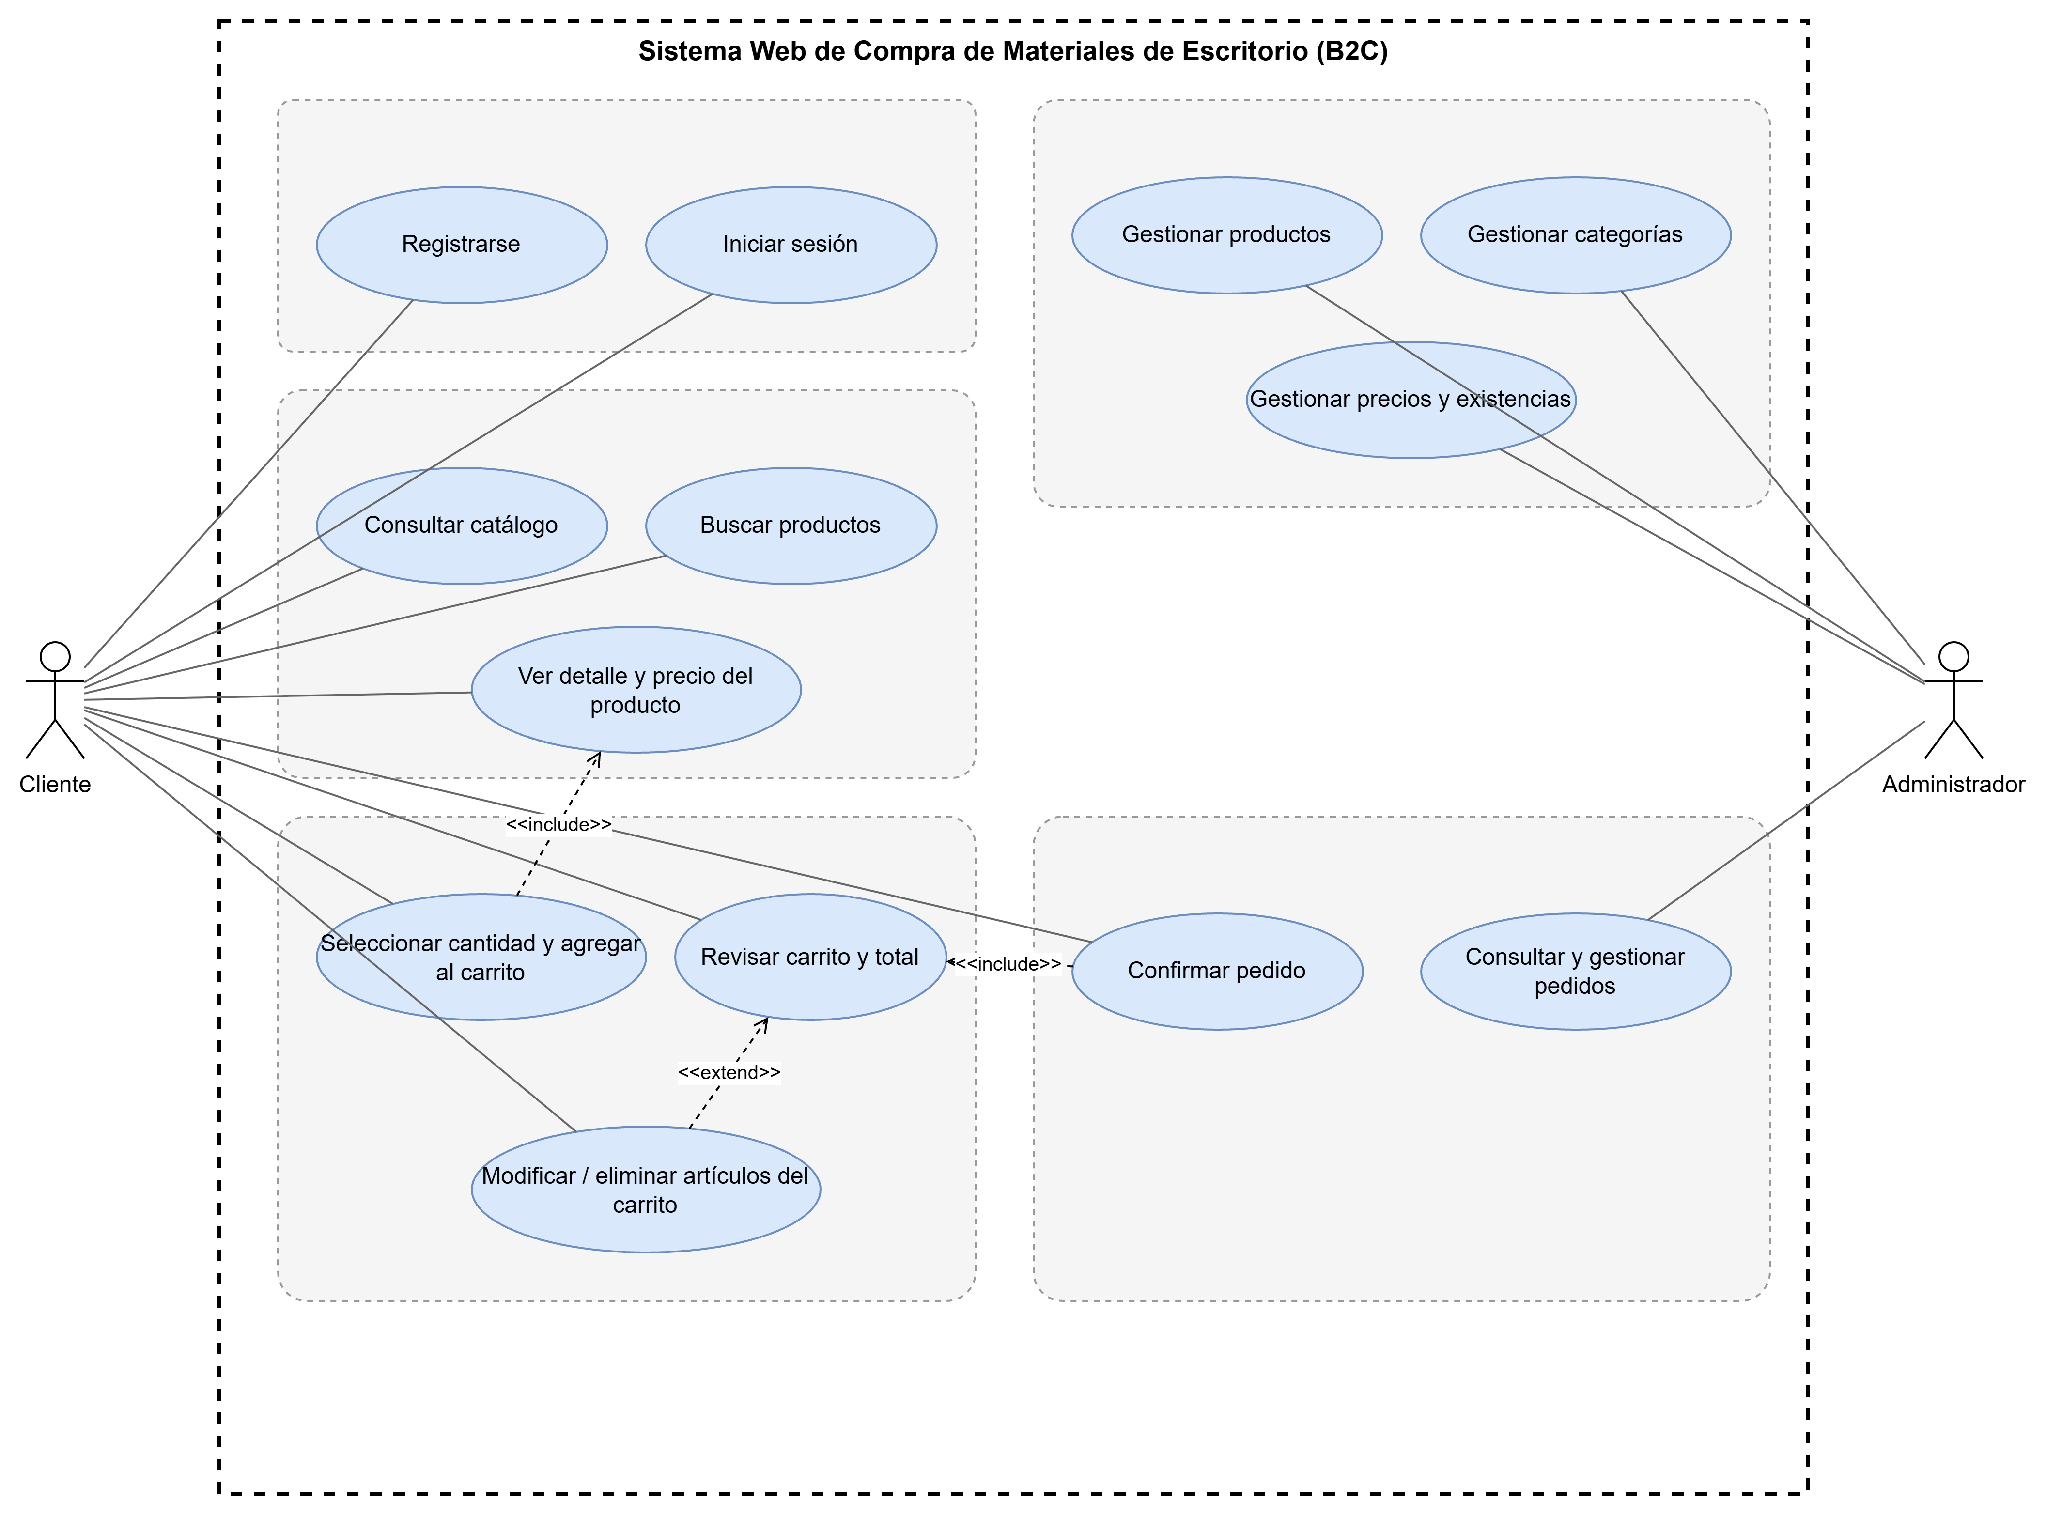
\includegraphics[width=1\textwidth]{diagrama_general.png}
    \caption{Diagrama de Casos de Uso General del Sistema Web de Compra de Materiales de Escritorio (B2C)}
    \label{fig:casos_uso_general}
\end{figure}
Como se ilustra en el diagrama general del sistema, el \textbf{Cliente} interactúa con los casos de uso de registro, inicio de sesión, consulta y búsqueda en el catálogo, visualización de detalles, gestión del carrito de compras (con relaciones \texttt{<<include>>} hacia la consulta de detalle y \texttt{<<extend>>} para modificar o eliminar artículos) y confirmación de pedidos. Por su parte, el \textbf{Administrador} gestiona productos, categorías, precios, existencias y la atención de pedidos.

A continuación, se detallan las especificaciones de los escenarios principales del sistema:

\subsubsection*{Caso de Uso 01: Gestionar Carrito de Compras y Confirmar Pedido}
\begin{itemize}
    \item \textbf{Actor Principal:} Cliente.
    \item \textbf{Precondición:} El cliente debe haber iniciado sesión (RF02) y estar visualizando el catálogo digital (RF04).
    \item \textbf{Flujo Normal:}
    \begin{enumerate}
        \item El cliente selecciona un producto del catálogo y pulsa la opción ``Agregar al carrito'' (RF08).
        \item El sistema verifica la disponibilidad de \textit{stock} en el inventario (RF11).
        \item El sistema añade el artículo al carrito y actualiza el contador de productos.
        \item El cliente ingresa al resumen del carrito, revisa los artículos seleccionados y modifica la cantidad de alguno de ellos (RF09).
        \item El sistema recalcula automáticamente los subtotales y el monto total a pagar (RF10).
        \item El cliente presiona ``Confirmar Pedido'' (RF12).
        \item El sistema valida nuevamente las existencias, genera un identificador único de pedido, descuenta el \textit{stock} del inventario y muestra un mensaje de confirmación.
    \end{enumerate}
    \item \textbf{Flujo Alternativo (Falta de Stock):} En el paso 2 o 7, si el sistema detecta que la cantidad solicitada supera las existencias disponibles, bloquea la operación y notifica al cliente que el producto se encuentra agotado o con unidades limitadas.
\end{itemize}

\subsubsection*{Caso de Uso 02: Gestionar Catálogo e Inventario}
\begin{itemize}
    \item \textbf{Actor Principal:} Administrador del Sistema.
    \item \textbf{Precondición:} El administrador ha iniciado sesión con sus credenciales autorizadas (RNF03).
    \item \textbf{Flujo Normal:}
    \begin{enumerate}
        \item El administrador accede al panel de administración de productos.
        \item Selecciona la opción ``Registrar nuevo producto'' (RF14).
        \item El sistema despliega el formulario de registro.
        \item El administrador completa los campos requeridos (nombre, categoría, descripción, precio unitario, \textit{stock} inicial e imagen referencial).
        \item El administrador pulsa ``Guardar''.
        \item El sistema valida la integridad de los datos (RNF08), almacena el registro en la base de datos y actualiza el catálogo visible para los clientes.
    \end{enumerate}
    \item \textbf{Flujo Alternativo (Datos Inválidos o Incompletos):} En el paso 6, si algún campo obligatorio (como el precio o el nombre) está vacío o contiene un formato incorrecto, el sistema resalta el campo y solicita su corrección antes de guardar.
\end{itemize}

\subsubsection*{Caso de Uso 03: Consultar y Actualizar Estado de Pedido}
\begin{itemize}
    \item \textbf{Actor Principal:} Cliente / Administrador del Sistema.
    \item \textbf{Precondición:} Existe al menos un pedido registrado previamente en el sistema (RF12).
    \item \textbf{Flujo Normal:}
    \begin{enumerate}
        \item El cliente ingresa a la sección ``Mis Pedidos'' en su perfil para consultar su historial (RF13), mientras que el administrador accede al módulo de ``Gestión de Pedidos'' (RF17).
        \item El administrador selecciona un pedido entrante, verifica los artículos solicitados y actualiza su estado (por ejemplo, de ``Recibido'' a ``En preparación'' o ``Entregado'').
        \item El sistema registra el cambio de estado y lo refleja en tiempo real en la vista de seguimiento del cliente.
    \end{enumerate}
\end{itemize}

\subsection{Evaluación de la Fase de Comunicación}

Al concluir las actividades de la Fase I bajo el enfoque metodológico AUP, el equipo de desarrollo establece las siguientes conclusiones evaluativas:

\begin{itemize}
    \item \textbf{Viabilidad técnica y operativa:} El proyecto es plenamente viable. La solución web bajo el modelo B2C responde directamente a la necesidad de digitalizar el catálogo de ``Suministros G\&T'', agilizar la toma de pedidos y reducir la dependencia de procesos manuales.
    \item \textbf{Calidad y trazabilidad de requerimientos:} Se definieron 18 requerimientos funcionales y 11 no funcionales claros, medibles y codificados, evitando ambigüedades mediante métricas concretas (como tiempos de respuesta y validaciones de inventario).
    \item \textbf{Delimitación temprana del alcance:} Se acordó desde esta etapa inicial que la primera versión del sistema no integrará pasarelas de pago en línea ni rastreo satelital de entregas, evitando desviaciones de alcance (\textit{scope creep}) y alineando las expectativas entre el equipo y el negocio.
    \item \textbf{Consenso y base documental:} La elaboración del glosario técnico y la especificación de los casos de uso proporcionan una base sólida y libre de ambigüedades para avanzar hacia las siguientes fases de Planeación y Modelado.
\end{itemize}

% --- Planificación ---
\section{Fase II: Planeación}

La fase de planeación establece el marco de trabajo con el que el equipo de siete integrantes desarrolla el Sistema Web de Compra de Materiales de Escritorio, orientado al modelo B2C (\textit{Business to Consumer}). En ella se delimita el alcance del proyecto, se estiman los recursos y el esfuerzo, se define el cronograma iterativo conforme al Proceso Unificado Ágil (AUP), se identifican y gestionan los riesgos mediante la estrategia RMMM de Pressman (Reducción, Supervisión y Gestión del Riesgo) y se establecen los mecanismos de seguimiento, el control de configuración y los criterios que determinan cuándo un entregable se considera terminado.

\subsection{Definición del Alcance y Delimitación del Proyecto}
\label{subsec:alcance_delimitacion}

Considerando la naturaleza y el alcance establecidos para el proyecto de asignatura, el trabajo se acota estrictamente hasta la etapa de diseño detallado y especificación técnica, bajo los siguientes límites:

\subsubsection*{Incluido en el alcance (Fases de Comunicación, Planeación y Modelado)}
\begin{itemize}
    \item \textbf{Ingeniería de Requerimientos y Alcance B2C:} Definición formal de actores, 18 requerimientos funcionales (\texttt{RF01}--\texttt{RF18}), 11 requerimientos no funcionales (\texttt{RNF01}--\texttt{RNF11}), glosario técnico y casos de uso generales y expandidos.
    \item \textbf{Modelado Estructural y de Datos:} Diagrama de clases del dominio y del sistema, modelo entidad-relación (E-R), esquema relacional normalizado y diccionario de datos en MySQL.
    \item \textbf{Modelado Dinámico y de Comportamiento:} Diagramas de secuencia, de actividades y de máquina de estados para los flujos críticos (registro, catálogo, carrito, validación de \textit{stock}, confirmación y gestión administrativa de pedidos).
    \item \textbf{Modelado Arquitectónico y Prototipado UX/UI:} Diagramas de componentes y de despliegue (arquitectura cliente-servidor web) y prototipos visuales navegables (\textit{wireframes} y \textit{mockups}) de las interfaces de Cliente y Administrador.
\end{itemize}

\subsubsection*{Excluido del alcance (fases posteriores y limitaciones funcionales)}
\begin{itemize}
    \item \textbf{Construcción y Despliegue (codificación):} No se contempla el desarrollo del código fuente productivo (Backend/Frontend), la puesta en marcha en servidores reales ni las pruebas de estrés en producción; estas actividades quedan proyectadas para una etapa posterior de implementación.
    \item \textbf{Pasarela de pagos electrónicos y rastreo GPS:} Dentro de la lógica modelada, los pedidos se confirman mediante la validación de disponibilidad en inventario y se gestionan por estados administrativos (\textit{Recibido}, \textit{En preparación}, \textit{En camino} y \textit{Entregado}), sin cobros en línea ni geolocalización.
\end{itemize}

Toda solicitud que exceda estos límites se tramita como solicitud de cambio, según el procedimiento de control de configuración establecido por el equipo.

\subsection{Estimación de Recursos}

Para ejecutar el proyecto dentro del calendario académico de la asignatura se asignan los siguientes recursos humanos, de hardware y de software.

\subsubsection{Recursos humanos (equipo de desarrollo: 7 integrantes)}

El equipo adopta una estructura colaborativa propia de AUP y concentra a la totalidad de sus integrantes en las disciplinas de análisis, modelado UML, diseño de datos y prototipado de interfaz. Cada artefacto tiene un responsable único y es revisado por un integrante distinto de su autor, tal como se detalla en la Tabla \ref{tab:roles_equipo}.

{\small
\begin{xltabular}{\textwidth}{|>{\raggedright\arraybackslash}p{2.8cm}|X|>{\raggedright\arraybackslash}p{3.6cm}|>{\raggedright\arraybackslash}p{1.8cm}|}
    % --- Título y encabezado de la PRIMERA página ---
    \caption{Roles, responsabilidades y artefactos del equipo}
    \label{tab:roles_equipo} \\
    \hline
    \textbf{Rol en el proyecto} & \textbf{Responsabilidades} & \textbf{Artefactos asociados} & \textbf{Iteraciones} \\
    \hline
    \endfirsthead

    % --- Encabezado que se repite en las páginas SIGUIENTES ---
    \multicolumn{4}{l}{\textit{Continuación de la Tabla \ref{tab:roles_equipo}}} \\
    \hline
    \textbf{Rol en el proyecto} & \textbf{Responsabilidades} & \textbf{Artefactos asociados} & \textbf{Iteraciones} \\
    \hline
    \endhead

    % --- Pie de tabla en páginas intermedias ---
    \multicolumn{4}{r}{\textit{Continúa en la siguiente página...}} \\
    \endfoot

    % --- Pie final de la tabla (con nota aclaratoria) ---
    \multicolumn{4}{l}{\footnotesize \textit{Nota:} En la Iteración 1 participa todo el equipo; el total de integrantes distribuidos por rol suma 7.} \\
    \endlastfoot

    % --- Contenido de las filas ---
    Líder de proyecto / coordinador & Planificación de iteraciones, seguimiento del cronograma, gestión de riesgos (RMMM), conducción de los \textit{check-ins} y consolidación del documento maestro. & Plan de proyecto, matriz RMMM e informe final. & I1 a I3 \\*
    \hline
    Especialistas en modelado dinámico & Especificación de casos de uso expandidos y elaboración de los diagramas de comportamiento del sistema. & Diagramas de casos de uso, secuencia, actividades y estados. & I1 a I3 \\*
    \hline
    Especialistas en modelado estructural y BD & Diseño de la estructura lógica del software, reglas de negocio de inventario y modelado de persistencia en MySQL. & Diagrama de clases, modelo E-R, modelo relacional normalizado y diccionario de datos. & I2 y I3 \\*
    \hline
    Especialista en arquitectura y UX/UI & Definición de la arquitectura cliente-servidor y diseño visual de las pantallas de Cliente y Administrador. & Diagramas de componentes y despliegue; \textit{wireframes} y \textit{mockups} en Figma. & I2 y I3 \\*
    \hline
    Responsable de calidad (QA de modelado y configuración) & Verificación de consistencia entre diagramas UML, trazabilidad con RF/RNF, administración del repositorio y control de versiones. & Matriz de trazabilidad, repositorio en GitHub, actas de revisión y de auditoría. & I1 a I3 \\
    \hline
\end{xltabular}
}

\subsubsection{Recursos de hardware y software}

\begin{itemize}
    \item \textbf{Hardware:} Computadoras personales (portátiles o de escritorio) de cada integrante, destinadas al diseño de modelos, la edición documental y el trabajo colaborativo en línea.
    \item \textbf{Software y herramientas (costo $\$0$, por uso académico o licencia abierta):}
    \begin{itemize}
        \item \textit{Modelado UML y de datos:} Draw.io (diagrams.net), estandarizado como herramienta única para los diagramas UML (casos de uso, clases, secuencia, actividades, estados, componentes y despliegue) y el modelo E-R, con archivos fuente en formato \texttt{.drawio}. Se emplea MySQL como motor de referencia para los tipos de datos del diccionario, únicamente a nivel de especificación.
        \item \textit{Prototipado de interfaces:} Figma, para \textit{wireframes} y pantallas de alta fidelidad (UX/UI).
        \item \textit{Documentación:} Overleaf (LaTeX) para la redacción técnica formal del documento maestro.
        \item \textit{Control de versiones y respaldo:} Git y GitHub como repositorio único de archivos fuente editables y de imágenes exportadas.
    \end{itemize}
\end{itemize}

\subsection{Estimación de Esfuerzo y Métricas del Proyecto}
\label{subsec:esfuerzo_metricas}

Dado que el esfuerzo del equipo se enfoca íntegramente en la ingeniería temprana y en el diseño detallado, se emplea la técnica de descomposición por artefactos de modelado y requerimientos.

\begin{itemize}
    \item \textbf{Tamaño funcional a modelar:} 18 requerimientos funcionales (\texttt{RF01}--\texttt{RF18}) y 11 requerimientos no funcionales (\texttt{RNF01}--\texttt{RNF11}), organizados en 4 módulos funcionales (Tabla \ref{tab:modulos_rf}). Los RNF son transversales a los cuatro módulos.
\end{itemize}

{\small
\begin{xltabular}{\textwidth}{|>{\raggedright\arraybackslash}p{3.5cm}|X|>{\raggedright\arraybackslash}p{3.0cm}|}
    % --- Título y encabezado de la PRIMERA página ---
    \caption{Módulos funcionales y requerimientos funcionales asociados}
    \label{tab:modulos_rf} \\
    \hline
    \textbf{Módulo funcional} & \textbf{Alcance} & \textbf{Requerimientos} \\
    \hline
    \endfirsthead

    % --- Encabezado que se repite en las páginas SIGUIENTES ---
    \multicolumn{3}{l}{\textit{Continuación de la Tabla \ref{tab:modulos_rf}}} \\
    \hline
    \textbf{Módulo funcional} & \textbf{Alcance} & \textbf{Requerimientos} \\
    \hline
    \endhead

    % --- Pie de tabla en páginas intermedias ---
    \multicolumn{3}{r}{\textit{Continúa en la siguiente página...}} \\
    \endfoot

    % --- Pie final de la tabla ---
    \endlastfoot

    % --- Contenido de las filas ---
    Acceso y Perfilamiento & Registro de clientes, inicio/cierre de sesión y gestión de perfiles. & RF01--RF03 (3) \\*
    \hline
    Catálogo Digital & Catálogo por categorías, clasificación, búsqueda y detalle de productos. & RF04--RF07 (4) \\*
    \hline
    Carrito y Pedidos & Carrito de compras, modificación, cálculo de importes, validación de disponibilidad, confirmación e historial de pedidos. & RF08--RF13 (6) \\*
    \hline
    Administración & Gestión de productos, categorías, precios, inventario (\textit{stock}), pedidos y cuentas de usuarios. & RF14--RF18 (5) \\*
    \hline
    \textbf{Total} & & \textbf{18 RF} \\
    \hline
\end{xltabular}
}

\begin{itemize}
    \item \textbf{Capacidad del equipo:} Con 7 integrantes que dedican entre $8$ y $10$ horas semanales al proyecto, la capacidad del equipo se sitúa entre $56$ y $70$ horas-persona por semana. Para planificar se adopta un valor de $65$ horas-persona por semana, lo que equivale a $195$ horas-persona totales en un ciclo de $3$ semanas.
    \item \textbf{Distribución porcentual del esfuerzo (enfoque en modelado):} Se presenta en la Tabla \ref{tab:distribucion_esfuerzo}.
\end{itemize}

{\small
\begin{xltabular}{\textwidth}{|X|>{\centering\arraybackslash}p{2.2cm}|>{\centering\arraybackslash}p{2.8cm}|>{\centering\arraybackslash}p{2.2cm}|}
    % --- Título y encabezado de la PRIMERA página ---
    \caption{Distribución del esfuerzo por fase}
    \label{tab:distribucion_esfuerzo} \\
    \hline
    \textbf{Fase} & \textbf{Esfuerzo} & \textbf{Horas-persona} & \textbf{Iteración} \\
    \hline
    \endfirsthead

    % --- Encabezado que se repite en las páginas SIGUIENTES ---
    \multicolumn{4}{l}{\textit{Continuación de la Tabla \ref{tab:distribucion_esfuerzo}}} \\
    \hline
    \textbf{Fase} & \textbf{Esfuerzo} & \textbf{Horas-persona} & \textbf{Iteración} \\
    \hline
    \endhead

    % --- Pie de tabla en páginas intermedias ---
    \multicolumn{4}{r}{\textit{Continúa en la siguiente página...}} \\
    \endfoot

    % --- Pie final de la tabla (con nota aclaratoria) ---
    \multicolumn{4}{l}{\footnotesize \textit{Nota:} Las horas se redondean al entero más cercano.} \\
    \endlastfoot

    % --- Contenido de las filas ---
    Fase I -- Comunicación (levantamiento y especificación de requerimientos) & $20\%$ & $39$ & I1 \\*
    \hline
    Fase II -- Planeación (alcance, estimación, cronograma y riesgos) & $15\%$ & $29$ & I1 \\*
    \hline
    Fase III -- Modelado (UML estructural, dinámico y arquitectónico, BD y prototipos) & $65\%$ & $127$ & I2 e I3 \\*
    \hline
    \textbf{Total} & \textbf{$100\%$} & \textbf{$195$} & \\
    \hline
\end{xltabular}
}

\subsubsection*{Métricas de seguimiento}
Para evaluar el avance y la calidad del proyecto se registran las siguientes métricas al cierre de cada iteración:
\begin{itemize}
    \item Porcentaje de artefactos planificados que cumplen la definición de terminado (Sección \ref{subsec:criterios_aceptacion}).
    \item Horas-persona reales frente a las planificadas, por fase e iteración.
    \item Cobertura de la matriz de trazabilidad: porcentaje de RF y RNF representados en los artefactos exigidos (meta: $100\%$).
    \item Hallazgos de la auditoría de consistencia: abiertos y cerrados, clasificados por severidad.
    \item Número de solicitudes de cambio recibidas y aprobadas sobre la línea base de requerimientos.
\end{itemize}

\subsection{Planificación Iterativa e Incremental (Cronograma AUP)}

Bajo el enfoque iterativo del Proceso Unificado Ágil (AUP), la primera semana se destina a consolidar las actividades de Comunicación y Planeación (fase de Inicio), y las dos semanas restantes se concentran de forma intensiva en los incrementos de la Fase III: Modelado (fase de Elaboración). Cada iteración concluye con una línea base (LB) verificada mediante la auditoría de consistencia descrita en la Sección \ref{subsec:seguimiento_control}.

{\footnotesize
\begin{xltabular}{\textwidth}{|>{\raggedright\arraybackslash}p{2.4cm}|>{\raggedright\arraybackslash}p{3.2cm}|X|>{\raggedright\arraybackslash}p{2.2cm}|>{\raggedright\arraybackslash}p{2.4cm}|}
    % --- Título y encabezado de la PRIMERA página ---
    \caption{Cronograma iterativo centrado en la Fase III: Modelado}
    \label{tab:cronograma_iterativo} \\
    \hline
    \textbf{Iteración, fase AUP y periodo} & \textbf{Objetivos} & \textbf{Entregables} & \textbf{Responsables clave} & \textbf{Hito de cierre} \\
    \hline
    \endfirsthead

    % --- Encabezado que se repite en las páginas SIGUIENTES ---
    \multicolumn{5}{l}{\textit{Continuación de la Tabla \ref{tab:cronograma_iterativo}}} \\
    \hline
    \textbf{Iteración, fase AUP y periodo} & \textbf{Objetivos} & \textbf{Entregables} & \textbf{Responsables clave} & \textbf{Hito de cierre} \\
    \hline
    \endhead

    % --- Pie de tabla en páginas intermedias ---
    \multicolumn{5}{r}{\textit{Continúa en la siguiente página...}} \\
    \endfoot

    % --- Pie final de la tabla (con nota aclaratoria) ---
    \multicolumn{5}{l}{\footnotesize \textit{Nota:} h-p: horas-persona planificadas. La auditoría de cada línea base se detalla en la Sección \ref{subsec:seguimiento_control}.} \\
    \endlastfoot

    % --- Contenido de las filas ---
    \textbf{Iteración 1} \newline Inicio (Comunicación y Planeación) \newline Semana 1 \newline $\approx 68$ h-p & Especificar requerimientos, delimitar el modelo B2C, planificar recursos, cronograma y riesgos, y preparar el repositorio y los estándares. & 
    \begin{itemize}[leftmargin=*, nosep]
        \item Actores, RF01--RF18, RNF01--RNF11 y glosario técnico.
        \item Diagrama general de casos de uso.
        \item Plan de proyecto y matriz RMMM.
        \item Repositorio GitHub y convenciones de nomenclatura.
    \end{itemize} & Coordinador, QA y todo el equipo. & \textbf{LB-I1:} Requerimientos y alcance aprobados; repositorio configurado. \\*
    \hline
    \textbf{Iteración 2} \newline Elaboración I (Modelado estructural y de datos) \newline Semana 2 \newline $\approx 64$ h-p & Especificar los casos de uso críticos, modelar la estructura lógica y la persistencia, e iniciar el prototipado. & 
    \begin{itemize}[leftmargin=*, nosep]
        \item Casos de uso expandidos de los flujos críticos.
        \item Diagramas de clases de análisis y de diseño.
        \item Modelo E-R, esquema relacional normalizado y diccionario de datos.
        \item \textit{Wireframes} iniciales de catálogo, carrito y panel administrativo.
        \item Matriz de trazabilidad v1.
    \end{itemize} & Especialistas estructurales y dinámicos, UX/UI y QA. & \textbf{LB-I2:} Modelo estructural y de datos auditado (auditoría 1). \\*
    \hline
    \textbf{Iteración 3} \newline Elaboración II (Modelado dinámico y arquitectónico) \newline Semana 3 \newline $\approx 63$ h-p & Modelar el comportamiento del sistema, definir la arquitectura, completar los prototipos y cerrar el documento maestro. & 
    \begin{itemize}[leftmargin=*, nosep]
        \item Diagramas de secuencia (registro, catálogo, carrito, validación de \textit{stock}, confirmación y gestión de pedidos).
        \item Diagramas de actividades y de estados del pedido y del carrito.
        \item Diagramas de componentes y despliegue (arquitectura web cliente-servidor).
        \item \textit{Mockups} navegables de Cliente y Administrador.
        \item Matriz de trazabilidad final, auditoría UML e informe final.
    \end{itemize} & Especialistas dinámicos, arquitectura y UX/UI, QA y Coordinador. & \textbf{LB-I3:} Informe final entregado; trazabilidad al $100\%$ (auditoría 2). \\
    \hline
\end{xltabular}
}

% =========================================================================
% INICIO DE BLOQUE PARA IMAGEN: CRONOGRAMA DE ITERACIONES Y LÍNEAS BASE
% Descomenta las siguientes líneas cuando tengas el archivo de imagen listo:
% =========================================================================
% \begin{figure}[H]
%     \centering
%     \includegraphics[width=0.95\textwidth]{cronograma_iteraciones.png}
%     \caption{Cronograma de las tres iteraciones y líneas base (LB)}
%     \label{fig:cronograma_iteraciones}
% \end{figure}

\subsection{Gestión de Riesgos (Estrategia RMMM)}

Siguiendo la metodología de Pressman para la Reducción, Supervisión y Gestión del Riesgo (RMMM), se identifican los riesgos propios de un proyecto centrado en el análisis y el modelado de software. Para cada riesgo se define una estrategia de mitigación (reducir la probabilidad o el impacto antes de que ocurra), una estrategia de supervisión (indicadores y momento de verificación) y un plan de contingencia (acción correctiva si el riesgo se materializa). La exposición de cada riesgo resulta de combinar su probabilidad con su impacto, según las escalas de la Tabla \ref{tab:escalas_riesgo}.

{\small
\begin{xltabular}{\textwidth}{|>{\raggedright\arraybackslash}p{2.6cm}|>{\raggedright\arraybackslash}p{3.4cm}|X|}
    % --- Título y encabezado de la PRIMERA página ---
    \caption{Escalas de probabilidad e impacto}
    \label{tab:escalas_riesgo} \\
    \hline
    \textbf{Nivel} & \textbf{Probabilidad} & \textbf{Impacto} \\
    \hline
    \endfirsthead

    % --- Encabezado que se repite en las páginas SIGUIENTES ---
    \multicolumn{3}{l}{\textit{Continuación de la Tabla \ref{tab:escalas_riesgo}}} \\
    \hline
    \textbf{Nivel} & \textbf{Probabilidad} & \textbf{Impacto} \\
    \hline
    \endhead

    % --- Pie de tabla en páginas intermedias ---
    \multicolumn{3}{r}{\textit{Continúa en la siguiente página...}} \\
    \endfoot

    % --- Pie final de la tabla ---
    \endlastfoot

    % --- Contenido de las filas ---
    Bajo / baja & Menor a $30\%$. & Retraso menor a un día o corrección local en un solo artefacto. \\*
    \hline
    Medio / media & Entre $30\%$ y $60\%$. & Retraso de uno a dos días o retrabajo en varios artefactos. \\*
    \hline
    Alto / alta & Mayor a $60\%$. & Compromete la entrega de una línea base o la consistencia global de los modelos. \\
    \hline
\end{xltabular}
}

\begin{figure}[H]
    \centering
    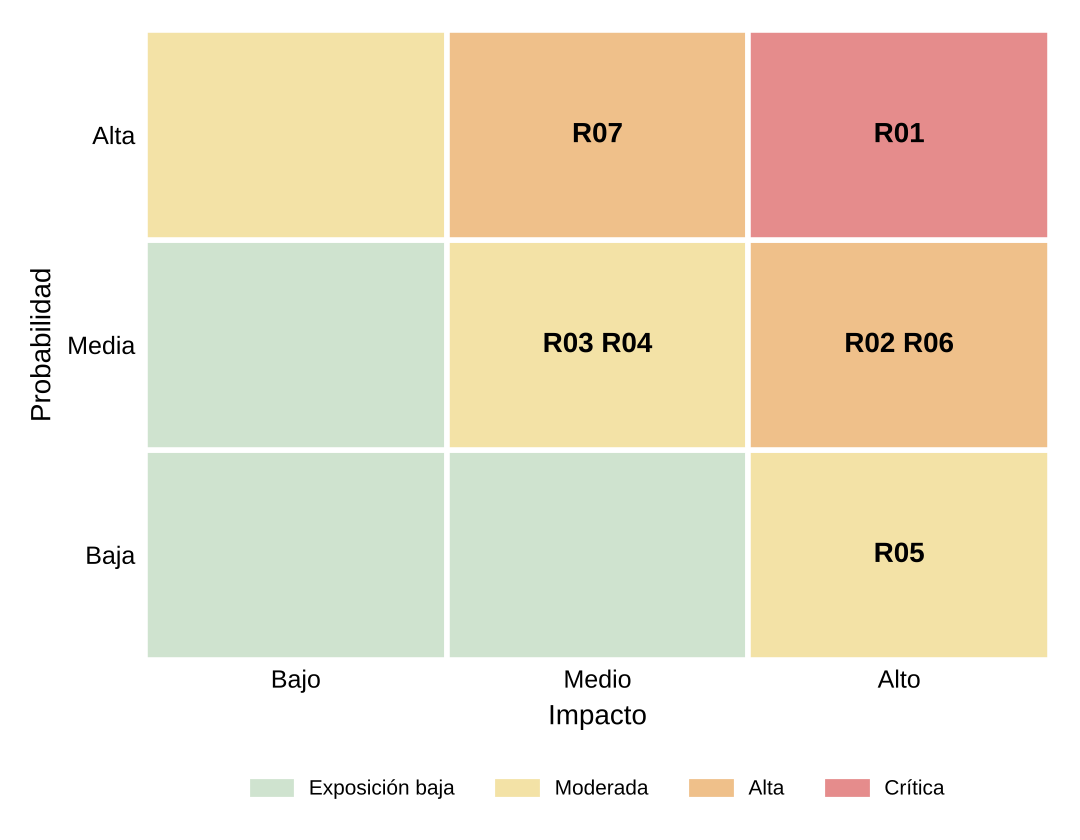
\includegraphics[width=0.75\textwidth]{matriz_exposicion_riesgos.png}
    \caption{Matriz de exposición de los riesgos R01--R07}
    \label{fig:matriz_exposicion_riesgos}
\end{figure}

La matriz detallada de identificación, análisis, mitigación, supervisión y contingencia se presenta a continuación en la Tabla \ref{tab:matriz_rmmm}.

{\scriptsize
\begin{xltabular}{\textwidth}{|>{\raggedright\arraybackslash}p{0.7cm}|>{\raggedright\arraybackslash}p{2.3cm}|>{\centering\arraybackslash}p{0.9cm}|>{\centering\arraybackslash}p{1.0cm}|X|X|X|>{\raggedright\arraybackslash}p{1.6cm}|}
    % --- Título y encabezado de la PRIMERA página ---
    \caption{Matriz de identificación, análisis y mitigación de riesgos enfocada en modelado}
    \label{tab:matriz_rmmm} \\
    \hline
    \textbf{ID} & \textbf{Descripción del riesgo} & \textbf{Prob.} & \textbf{Imp.} & \textbf{Mitigación} & \textbf{Supervisión} & \textbf{Contingencia} & \textbf{Resp.} \\
    \hline
    \endfirsthead

    % --- Encabezado que se repite en las páginas SIGUIENTES ---
    \multicolumn{8}{l}{\textit{Continuación de la Tabla \ref{tab:matriz_rmmm}}} \\
    \hline
    \textbf{ID} & \textbf{Descripción del riesgo} & \textbf{Prob.} & \textbf{Imp.} & \textbf{Mitigación} & \textbf{Supervisión} & \textbf{Contingencia} & \textbf{Resp.} \\
    \hline
    \endhead

    % --- Pie de tabla en páginas intermedias ---
    \multicolumn{8}{r}{\textit{Continúa en la siguiente página...}} \\
    \endfoot

    % --- Pie final de la tabla ---
    \endlastfoot

    % --- Contenido de las filas ---
    \textbf{R01} & Inconsistencia de nombres, atributos o métodos entre el diagrama de clases, los diagramas de secuencia y el modelo E-R. & Alta & Alto & Usar el glosario y el diccionario de datos como fuente única de nombres; realizar revisiones cruzadas lideradas por QA antes de cerrar cada iteración. & Lista de verificación de nomenclatura en cada auditoría; conteo de hallazgos por iteración (meta: cero críticos abiertos). & Congelar el diagrama afectado, tomar el diccionario de datos como referencia y corregir en una sesión conjunta de hasta un día. & QA \\*
    \hline
    \textbf{R02} & Ambigüedad en las reglas de negocio críticas (p. ej., descuento de \textit{stock} al confirmar el pedido o estados del pedido). & Media & Alto & Documentar precondiciones, postcondiciones y flujos alternativos en los casos de uso expandidos antes de elaborar las secuencias. & Revisión de los casos de uso expandidos por especialistas dinámicos y estructurales; registro de dudas abiertas en el acta de cada \textit{check-in}. & Adoptar provisionalmente la interpretación del Coordinador, documentarla como supuesto y revalidarla en la siguiente auditoría. & Coordinador y especialistas dinámicos \\*
    \hline
    \textbf{R03} & Desviación del alcance (\textit{scope creep}) al intentar programar prototipos funcionales en lugar de profundizar el modelado. & Media & Medio & Mantener el enfoque en los artefactos UML, el diseño de BD y los \textit{mockups} estáticos o navegables acordados en la Sección \ref{subsec:alcance_delimitacion}. & Contrastar en cada \textit{check-in} las tareas en curso con el cronograma y el alcance; vigilar la aparición de código en el repositorio. & Suspender la tarea fuera de alcance, retirarla de la rama principal y reasignar sus horas a artefactos pendientes. & Coordinador \\*
    \hline
    \textbf{R04} & Diferencias de notación UML o de estilo visual al dividir los diagramas entre los 7 integrantes. & Media & Medio & Estandarizar Draw.io como única herramienta, además de la paleta de colores y las convenciones de nomenclatura, desde la semana 1; publicar una plantilla base en el repositorio. & Revisión de notación y estilo en la auditoría de cada iteración. & Homogeneizar los diagramas con la plantilla; QA asigna la tarea a un integrante por iteración. & QA y arquitectura \\*
    \hline
    \textbf{R05} & Pérdida o desactualización de los archivos editables de diagramas o del documento. & Baja & Alto & Centralizar todos los archivos fuente (\texttt{.drawio}, \texttt{.tex} y exportaciones) en el repositorio GitHub, con \textit{commits} al cierre de cada sesión de trabajo. & QA verifica en cada \textit{check-in} que el último \textit{commit} refleje el avance reportado. & Restaurar la última versión desde el historial de Git o la copia local; reconstruir desde las exportaciones PNG/PDF si es necesario. & QA \\*
    \hline
    \textbf{R06} & Cambios o interpretaciones divergentes de los RF/RNF tras aprobarse la línea base de requerimientos (p. ej., lecturas distintas de RF11 y RF12). & Media & Alto & Congelar los requerimientos en LB-I1; tramitar todo cambio como solicitud de cambio; mantener actualizada la matriz de trazabilidad. & Comparar la matriz de trazabilidad con la versión vigente de los RF/RNF en cada auditoría; llevar el registro de solicitudes de cambio. & Evaluar el impacto con la matriz de trazabilidad, actualizar solo los artefactos afectados y generar una nueva versión con su acta. & Coordinador y QA \\*
    \hline
    \textbf{R07} & Conflictos de edición o sobrescritura de archivos de diagramas por el trabajo concurrente de varios integrantes. & Alta & Medio & Asignar un responsable único por artefacto; trabajar en ramas por artefacto y fusionar mediante \textit{pull request}; aplicar la convención de nombres de archivo. & Revisar en cada \textit{check-in} el historial de \textit{commits} y los conflictos de fusión reportados. & Resolver el conflicto desde el historial de Git conservando la versión de la línea base más reciente y reaplicar manualmente los cambios perdidos. & QA \\
    \hline
\end{xltabular}
}

\subsection{Mecanismos de Seguimiento y Control del Proyecto}
\label{subsec:seguimiento_control}

Para garantizar la calidad técnica de los modelos y el cumplimiento del cronograma de 3 semanas, el equipo aplica tres mecanismos de control complementarios: uno operativo (reuniones de sincronización), uno de verificación (auditoría de consistencia) y uno de cobertura (matriz de trazabilidad). Sus resultados alimentan la supervisión de la matriz RMMM y las métricas de la Sección \ref{subsec:esfuerzo_metricas}.

\subsubsection{Reuniones de sincronización cortas (\textit{check-ins})}
Sesiones breves de 15 minutos, realizadas cada dos días (aproximadamente diez en el ciclo de 3 semanas), conducidas por el Coordinador. Cada integrante informa qué avanzó, qué hará hasta la siguiente sesión y qué impedimentos tiene. Sirven para revisar el avance de cada diagrama, resolver dudas de lógica de negocio y evitar trabajo duplicado entre los 7 integrantes. Los acuerdos, los impedimentos y las dudas abiertas se registran en un acta breve almacenada en el repositorio; los impedimentos que persistan más de dos sesiones se escalan al Coordinador y se incorporan a la supervisión de riesgos.

\subsubsection{Auditoría de consistencia UML al cierre de cada iteración}
Revisión conjunta, liderada por el responsable de QA, en la que se verifica que cada clase, entidad y mensaje de los diagramas de secuencia coincida exactamente en nomenclatura y cardinalidad con el resto de los artefactos. Se aplica una lista de verificación que incluye: correspondencia entre clases, entidades y tablas; coincidencia de los mensajes de secuencia con métodos de clase; coherencia de los estados del pedido (\textit{Recibido}, \textit{En preparación}, \textit{En camino} y \textit{Entregado}) en los diagramas de actividades y de estados; y cumplimiento de la notación y de la plantilla visual. Los hallazgos se clasifican por severidad (crítico, mayor o menor) y se registran en el acta de auditoría con su responsable y su estado; no se cierra la línea base de la iteración mientras existan hallazgos críticos abiertos.

\subsubsection{Matriz de trazabilidad requerimiento-modelo}
Control cruzado que asegura que los 18 requerimientos funcionales (\texttt{RF01}--\texttt{RF18}) y los 11 no funcionales (\texttt{RNF01}--\texttt{RNF11}) estén debidamente representados en los artefactos de modelado. Cada RF debe vincularse al menos con un caso de uso, un elemento del modelo estructural o de datos, un diagrama dinámico y una pantalla del prototipo. Cada RNF debe vincularse al menos con un artefacto de diseño que lo atienda (arquitectura, modelo de datos o prototipo). QA crea la matriz en la Iteración 2, la actualiza al cierre de cada iteración y la utiliza para evaluar el impacto de las solicitudes de cambio; la cobertura esperada al cierre del proyecto es del $100\%$.

{\small
\begin{xltabular}{\textwidth}{|>{\raggedright\arraybackslash}p{3.4cm}|>{\raggedright\arraybackslash}p{3.0cm}|>{\raggedright\arraybackslash}p{2.4cm}|X|}
    % --- Título y encabezado de la PRIMERA página ---
    \caption{Resumen de los mecanismos de seguimiento y control}
    \label{tab:mecanismos_control} \\
    \hline
    \textbf{Mecanismo} & \textbf{Frecuencia} & \textbf{Responsable} & \textbf{Insumo} \\
    \hline
    \endfirsthead

    % --- Encabezado que se repite en las páginas SIGUIENTES ---
    \multicolumn{4}{l}{\textit{Continuación de la Tabla \ref{tab:mecanismos_control}}} \\
    \hline
    \textbf{Mecanismo} & \textbf{Frecuencia} & \textbf{Responsable} & \textbf{Insumo} \\
    \hline
    \endhead

    % --- Pie de tabla en páginas intermedias ---
    \multicolumn{4}{r}{\textit{Continúa en la siguiente página...}} \\
    \endfoot

    % --- Pie final de la tabla ---
    \endlastfoot

    % --- Contenido de las filas ---
    \textit{Check-ins} de sincronización & Cada 2 días (15 min) & Coordinador & Avance individual, impedimentos y dudas. \\*
    \hline
    Auditoría de consistencia UML & Al cierre de cada iteración (3) & QA & Diagramas, glosario, diccionario de datos y lista de verificación. \\*
    \hline
    Matriz de trazabilidad & Actualización al cierre de cada iteración & QA & RF/RNF vigentes y artefactos de cada iteración. \\
    \hline
\end{xltabular}
}

\subsection{Criterios de Aceptación y Definición de Terminado}
\label{subsec:criterios_aceptacion}

Los criterios de aceptación establecen las condiciones que debe cumplir cada entregable para ser admitido en una línea base, y la definición de terminado (DoD, \textit{Definition of Done}) fija las condiciones comunes que debe satisfacer cualquier artefacto, iteración y el proyecto en su conjunto.

\subsubsection{Criterios de aceptación por entregable}

{\footnotesize
\begin{xltabular}{\textwidth}{|>{\raggedright\arraybackslash}p{3.0cm}|X|>{\raggedright\arraybackslash}p{2.6cm}|}
    % --- Título y encabezado de la PRIMERA página ---
    \caption{Criterios de aceptación de los entregables}
    \label{tab:criterios_aceptacion} \\
    \hline
    \textbf{Entregable} & \textbf{Criterio de aceptación} & \textbf{Verifica} \\
    \hline
    \endfirsthead

    % --- Encabezado que se repite en las páginas SIGUIENTES ---
    \multicolumn{3}{l}{\textit{Continuación de la Tabla \ref{tab:criterios_aceptacion}}} \\
    \hline
    \textbf{Entregable} & \textbf{Criterio de aceptación} & \textbf{Verifica} \\
    \hline
    \endhead

    % --- Pie de tabla en páginas intermedias ---
    \multicolumn{3}{r}{\textit{Continúa en la siguiente página...}} \\
    \endfoot

    % --- Pie final de la tabla ---
    \endlastfoot

    % --- Contenido de las filas ---
    Requerimientos y glosario & 18 RF y 11 RNF identificados de forma única, redactados de manera verificable y sin contradicciones; glosario con los términos de negocio utilizados en los demás artefactos; alcance B2C sin pasarela de pagos ni rastreo GPS. & QA y Coordinador \\*
    \hline
    Casos de uso & Diagrama general con los actores Cliente y Administrador que cubre los 4 módulos; casos expandidos de los flujos críticos con actor, precondiciones, flujo principal, flujos alternativos y postcondiciones. & Especialistas dinámicos y QA \\*
    \hline
    Diagrama de clases & Clases, atributos, métodos y multiplicidades definidos; reglas de inventario y validación de disponibilidad (RF11) reflejadas; nombres coherentes con el glosario y el modelo E-R. & Especialistas estructurales y QA \\*
    \hline
    Modelo E-R, esquema relacional y diccionario de datos & Entidades, claves primarias y foráneas y cardinalidades definidas; esquema normalizado al menos hasta tercera forma normal; diccionario con tipo de dato MySQL, longitud, restricciones y descripción de cada atributo. & Especialistas estructurales y QA \\*
    \hline
    Diagramas de secuencia, actividades y estados & Cubren los flujos críticos de registro, catálogo, carrito, validación de \textit{stock}, confirmación y gestión de pedidos; los mensajes corresponden a métodos de clase; los estados del pedido (\textit{Recibido}, \textit{En preparación}, \textit{En camino} y \textit{Entregado}) tienen transiciones válidas. & Especialistas dinámicos y QA \\*
    \hline
    Diagramas de componentes y despliegue & Representan la arquitectura cliente-servidor web con sus capas de presentación, lógica y datos, y atienden al menos los RNF de seguridad, compatibilidad y mantenibilidad (RNF03, RNF06 y RNF09). & Arquitectura y QA \\*
    \hline
    Prototipos (\textit{wireframes} y \textit{mockups}) & Pantallas de Cliente y Administrador navegables, que cubren todas las funciones con interfaz de usuario de los RF, incluidos los mensajes de validación de disponibilidad; diseño adaptable a distintos tamaños de pantalla (RNF07) y estilo visual consistente. & UX/UI y QA \\*
    \hline
    Matriz de trazabilidad & Cobertura del $100\%$: cada RF vinculado a un caso de uso, un elemento estructural o de datos, un diagrama dinámico y una pantalla; cada RNF vinculado a un artefacto de diseño. & QA \\*
    \hline
    Informe final & Documento maestro integrado, con numeración y referencias de figuras y tablas, ortografía y puntuación revisadas y etiqueta \texttt{LB-I3} en el repositorio. & Coordinador y QA \\
    \hline
\end{xltabular}
}

\subsubsection{Definición de terminado de un artefacto}
Un artefacto se considera terminado cuando cumple todas las condiciones siguientes:
\begin{enumerate}
    \item Satisface los criterios de aceptación de su entregable (Tabla \ref{tab:criterios_aceptacion}).
    \item Emplea la notación UML, la nomenclatura y la plantilla visual estandarizadas por el equipo.
    \item Fue revisado por un integrante distinto de su autor y cuenta con el visto bueno de QA.
    \item No tiene hallazgos críticos ni mayores abiertos en la auditoría de consistencia.
    \item Su trazabilidad con los RF/RNF está registrada y actualizada en la matriz.
    \item Su fuente editable y su exportación (PNG / PDF) están en el repositorio, en versión 1.0 y fusionadas mediante \textit{pull request} aprobado.
    \item Está incluido en el documento maestro con leyenda, numeración y referencia en el texto.
\end{enumerate}

\subsubsection{Definición de terminado de una iteración y del proyecto}
\begin{itemize}
    \item \textbf{Iteración:} Todos los artefactos planificados cumplen la definición de terminado; la auditoría de consistencia se realizó y su acta está archivada; la matriz de trazabilidad y la matriz RMMM están actualizadas; y la etiqueta de línea base (\texttt{LB-I1}, \texttt{LB-I2} o \texttt{LB-I3}) fue creada.
    \item \textbf{Proyecto:} Las tres líneas base están cerradas; los 18 RF y los 11 RNF cuentan con cobertura del $100\%$ en la matriz de trazabilidad; el informe final fue entregado; y no se produjo ningún elemento de los excluidos en la Sección \ref{subsec:alcance_delimitacion}.
\end{itemize}

\end{document}